\chapter{Erstellung des Datensatzes} \label{ch 6}
\section{Datenbeschaffung durch Web Scraping}

Um die erste Forschungsfrage zu beantworten, muss ein Korpus erstellt werden, für deutsche Clickbaits. Für die Erstellung eines solchen Korpus sind zunächst bestimmte Seiten einzugrenzen, die Clickbait Nachrichten anbieten. Die bekannteste Seite ist \enquote{buzzfeed}\footnote{Beinhaltet außerdem Schlagzeilen aus den Unterseiten \enquote{tasty} und \enquote{quiz}}. Außerdem wurden auch Webseiten wie \enquote{web.de} oder \enquote{tv-movie} nach Clickbaits gescannt. Das Screening wurde am November 2020 durchgeführt. Um jedoch zu gewährleisten, dass die Nachrichten zeitlich weit auseinander liegen und somit eine größere Diversität haben, wurden Webseiten ausgewählt die Ihre Nachrichten in gewisser Weise Archivieren. Die gesammelten Daten reichen teilweise über ein Jahr zurück. Wie im Listing~\ref{Scrapy} in Zeile 12 zu sehen ist, besitzt die Seite im Beispiel eine Pagination-Funktion. Dieses Pagination reicht in eine weite Vergangenheit zurück.

\begin{table}[h]
    \caption{Vergleich der Anzahl und Herkunft Rohdaten nach dem Scrapingvorgang}
    \label{Datensatz_Herkunft}
    \renewcommand{\arraystretch}{1.2}
    \centering
    \sffamily
    \begin{footnotesize}
        \begin{tabular}{l l l}
            \toprule
            \textbf{Quelle}   & \textbf{Methodik} & Elemente \\
            \midrule
            de.wikinews.org   & API-Zugang        & 10.612   \\
            web.de            & Web Scraping      & 14.163   \\
            tvmovie.de        & Web Scraping      & 9.428    \\
            buzzfeed.de       & Web Scraping      & 798      \\
            promipool.de      & Web Scraping      & 26.779   \\
            heftig.de         & Web Scraping      & 605      \\
            frauenseite.net   & Web Scraping      & 148      \\
            bravo.de          & Web Scraping      & 7.476    \\
            \midrule
            Summe Clickbaits  &                   & 59.407   \\
            Summe Nachrichten &                   & 10.612   \\
            Summe insgesamt   &                   & 70.019   \\
            \bottomrule
        \end{tabular}
    \end{footnotesize}
    \rmfamily
\end{table}



Das Verfahren wurde automatisch mittels eines programmierten Scrapers je Seite durchgeführt. Ein Scraper ist ein Programm, welches Informationen aus einer Webseite automatisch extrahieren kann. Dieses gelingt, indem es nach HTML- oder CSS-Attributen oder sogar AJAX-Anfragen durchsucht oder diese imitiert. Im Listing~\ref{Scrapy} wird ein Web-Scraper vorgestellt. Scrapy führt in einer Schleife HTTP-Requests durch welche jeweils eine Antwort bekommen. Es können auch AJAX-Anfragen gesendet werden (z.B. ein POST-Request). Wenn die Anfrage Erfolgreich ist, kann die daraus resultierende Antwort auf bestimmte Eigenschaften und Attribute durchsucht werden (im Beispiel werden CSS-Attribute durchsucht). Diese Attribute beinhalten meisten die gewünschte Information, welches dann wie in der \texttt{parse\_url} und \texttt{parse\_page} Methode gezogen und in eine Datenbank gespeichert wird.



\begin{lstlisting}[language=Python,caption=Beispiel eines Scrapers,label={Scrapy}]
import scrapy
from scrapy.http.request import Request
from datetime import datetime
from klickscraper.items import WebdeItem


class WebdeSpider(scrapy.Spider):
    name = "webde"
    scraped_at = datetime.now()

    def start_requests(self):
        for i in range(287):
            url = f"https://web.de/magazine/unterhaltung/stars/p{i}"
            yield Request(
                dont_filter=True,
                callback=self.parse_url,
                url=url)

    def parse_url(self, response):
        follow_ulrs = response.css(
            ".teaser-article__full").css("a::attr(href)").getall()
        for f in follow_ulrs:
            yield Request(
                url=f,
                dont_filter=True,
                callback=self.parse_page)

    def parse_page(self, response):
        if len(response.css("p::text").getall()) > 10:
            text = " ".join(response.css("p::text").getall())
        else:
            text = None
        yield WebdeItem(title=response.css("title::text").get(),
                        text=text,
                        scraped_at=self.scraped_at)
\end{lstlisting}


\section{Rohdatenanalyse}
Um aus den Rohdaten Schlüsse über die sprachlichen Eigenschaften zu ziehen wird im folgenden Abschnitt eine explorative Rohdatenanalyse durchgeführt. Um dies möglichst zu vereinfachen, wird der Rohdatensatz, welches in einer SQL-Datenbank gespeichert wurde in ein Pandas\footnote{Pandas ist ein schnelles, flexibles und benutzerfreundliches Open-Source-Tool zur Analyse und Bearbeitung von Daten in Python.} Dataframe umgewandelt.
Aus der Abbildung \ref{Kap5:Hist2} ist zu sehen, dass die Wortlänge in den Schlagzeilen der Wikinews Schlagzeilen länger ist. Dieses Phänomen war nach der Literaturanalyse aus Kapitel \ref{ch4} zu erwarten. Neben der Länge der Wörter aus den Schlagzeilen, ist auch die Analyse der Wortauswahl relevant. Aus der Literaturstudie können bestimmte Merkmale von Clickbaits festgestellt werden. Clickbaits enthalten meistens eine Frage oder Zahlen. Außerdem ist bei Clickbaits auch eine gewisse Wortauswahl festzustellen. Die Zuordnung der Wörter je Clickbait-Schlagzeile zu den Wortarten (Part-of-speech-Tagging oder POS-Tagging) wurde mittels der Python NLP-Bibliothek Spacy durchgeführt. Auch hier wurden Erkenntnisse aus Kapitel \ref{ch4} berücksichtigt. Die Ergebnisse dieser Analyse sind aus der Tabelle~\ref{pos} zu entnehmen.

\begin{table}[h]
    \caption{Vergleich der Ergebnisse des POS-Taggings}
    \label{pos}
    \renewcommand{\arraystretch}{1.2}
    \centering
    \sffamily
    \begin{footnotesize}
        \begin{tabular}{l l l}
            \toprule
            \textbf{TAG}                  & \textbf{Auffälliges Wort (Häufigkeit)} \\
            \midrule
            ADJA  (attributives Adjektiv) & neu (1759), neue (1474)                \\
            ADJD   (adverbiales Adjektiv) & krass (171), wirklich  (349)           \\
            ADV   (Adverb)                & so (5142), endlich (357)               \\
            PDAT (Demonstrativpronomen)   & dies (3566)                            \\
            PROAV   (Pronominaladverb)    & darum (588), deshalb (251)             \\
            PWAT (Interrogativpronomen)   & welch (154)                            \\
            PWAV  (Relativpronomen)       & wie (488) warum (184)                  \\
            \bottomrule
        \end{tabular}
    \end{footnotesize}
    \rmfamily
\end{table}


\begin{figure}[H]
    \centering
    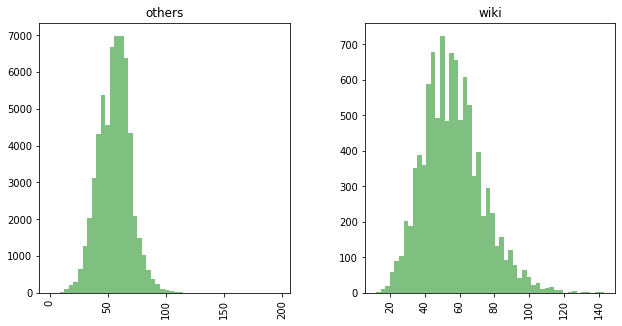
\includegraphics[width=14cm]{kapitel5/hist1wikicl.png}
    \caption[Vergleich der Wortlängen der Schlagzeilen aus den Rohdaten]{Die Rohdatenanalyse zeigt, dass das Histogramm rechts (Wikinews) eine höhere Varianz hat, als das Histogramm links (Clickbaits).}
    \label{Kap5:Hist2}
\end{figure}



\section{Labeln der Daten}\label{secLabel}
Aus der Tabelle~\ref{Datensatz_Herkunft} ist zu entnehmen, dass ca. 60.000 potenzielle Clickbaits vorhanden sind. Es wird angestrebt einen Datensatz in der Größenordnung von 10.000 - 20.000 Schlagzeilen zu generieren. Mit den 10.000 Wikinews Artikeln ist die erste Hälfte des Datensatzes praktisch vorhanden. An diesem Datensatz muss nichts mehr gelabelt werden, da angenommen wird, dass diese Nachrichten einen Standard haben, sodass diese als Nicht-Clickbaits gekennzeichnet werden. Fraglich ist jedoch, ob nur die Auswahl eines Mediums ausreichend ist. Um die restlichen 10.000 Schlagzeilen, also die Clickbaits zu ermitteln, bietet sich die Möglichkeit, die Daten per Hand zu kennzeichnen. Diese Aufgabe nimmt jedoch relativ viel Ziel in Anspruch, sodass für diese Aufgabe ein \enquote{regelbasiertes Labeln} ausgeführt werden kann. Bestimmte Muster und Eigenschaften können durch Techniken der NLP programmatisch erkannt und somit das Labeln automatisiert werden. Fraglich ist jedoch, die Qualität dieses Ansatzes. Dieser Ansatz kann das menschliche Labeln natürlich nicht ersetzen und sollte wenn Möglich erweitert und verbessert werden.

Es können folgende Muster und Eigenschaften erkannt werden:

\begin{enumerate}
    \item Clickbaits sind meistens Fragen wie \enquote{Welcher Schuh passt dir am meisten?}
    \item Clickbaits enthalten meistens Zahlen in Form eines Listings \enquote{Das sind die 10 schnellsten Autos}
    \item Clickbaits haben eine niedrigere Wortlänge als normale Nachrichten
    \item Clickbaits beinhalten einige für sie markanten Wörter wie \enquote{diese} oder \enquote{so}
\end{enumerate}

Diese Erkenntnisse können programmatisch umgewandelt werden und somit der Rohdatensatz um ein vielfaches reduziert werden. Somit braucht es zunächst kein händisches Labeln der Daten, da dieser Prozess völlig automatisch erfolgt. Der Nachteil dieses Verfahrens ist, dass die Daten falsche Positive haben können und evtl. nicht Präzise genug sind. Im folgenden werden die Ansätze die oben beschrieben wurden in Python-Code transformiert. Die Funktion aus Listing \ref{Label1} kann z.B. dafür verwendet werden, um den Datensatz nach bestimmten Kriterien wie \enquote{Beinhaltet die Schlagzeile ein Fragezeichen oder eine Zahl} zu filtern. Ebenfalls kann die Wortlänge durch die Funktion aus Listing \ref{Label2} ermittelt werden. Mit der Funktion aus Listing \ref{Label3} können bestimmte Tags ermittelt und der Titel nach dem Vorhandensein dieser Tags gefiltert werden. 


\begin{lstlisting}[language=Python,caption=Die Funktion labelt nach bestimmten Kriterien den Datensatz, label={Label1}]
def contains_word(word, row):
    for r in row:
        if r in word:
            return 1


def label_data_with_arg(df, col_name, arg_):
    return df[col_name].apply(
        lambda x: contains_word(arg_, re.findall(r"[\w']+|[.,!?;]", x.lower())))
\end{lstlisting}

\begin{lstlisting}[language=Python,caption=Funktionen die die durchschnittliche Wortlänge erkennen und nach Interpunktion filtern, label={Label2}]
import re
import string


def remove_punc(text):
    text = re.sub("\[.*?\]", "", text)
    text = re.sub("https?://\S+|www\.\S+", "", text)
    text = re.sub("<.*?>+", "", text)
    text = re.sub("[%s]" % re.escape(string.punctuation), "", text)
    text = re.sub("\n", "", text)
    text = re.sub("\w*\d\w*", "", text)
    return text

def get_avg_length(string):
    words = remove_punc(string).split()
    try:
        count = int(sum(len(word) for word in words) / len(words))
    except ZeroDivisionError:
        count = 1
    return count
\end{lstlisting}

\begin{lstlisting}[language=Python,caption=Tagger Funktion, welches den Text nach der Grammatik filtert, label={Label3}]
import spacy
nlp = spacy.load("de")


def contains_pos(sentence):
    list_ = ["PDAT", "ADJD", "ADJA", "PIS", "PWAV", 
            "PTKA", "VAFIN", "PROAV", "ADV"]
    doc = nlp(sentence)
    for token in doc:
        if str(token.tag_) in list_:
            return 1

def label_data_with_pos(df, col_name):
    return df[col_name].apply(
        lambda x: contains_pos(x.lower()))
\end{lstlisting}


\section{Analyse der Daten}\label{sectionAnalyse}
Die Summe der Wikinews Nachrichten beträgt ca. 10.000. Mit der Zugabe weiterer 10.000 Clickbaits, die durch das labeln entstehen, ergibt sich ein Datensatz mit 20.000 Beispielen. Die Tabelle~\ref{data} verschafft einen Überblick über alle Daten. Interessant ist dabei, dass bei den Clickbaits ca. 33\% aller Clickbaits ein Fragezeichen oder eine Zahl beinhalten und ca. die Hälfte aller Daten im Datensatz ein bestimmtes Tag wie \enquote{diese} oder \enquote{so} enthalten. Bei den Wikinews Nachrichten liegen diese Anteile sehr weit unten. Die durchschnittliche Wortlänge beträgt bei den Clickbaits bei 5, während bei den Wikipedia Nachrichten dieses bei 7 liegt.
Bei der Betrachtung der Wörter mit der Word-Cloud Analyse können bestimmte Themen erkannt werden. Auffällig bei den Clickbaits sind neben \enquote{Promis} auch die Wörter \enquote{darum}, \enquote{quiz} \enquote{sieht} und \enquote{macht}. Bei den Wikipedia Nachrichten geht es mehr um Deutschland und der Welt.


\begin{table}[h]
    \caption{Beschreibung des gelabelten Datensatzes}
    \label{data}
    \renewcommand{\arraystretch}{1.2}
    \centering
    \sffamily
    \begin{footnotesize}
        \begin{tabular}{l l l l l l}
            \toprule
                           & \textbf{has\_question} & \textbf{has\_keyword} & \textbf{has\_number} & \textbf{avg\_word\_length} & \textbf{label} \\
            \textbf{count} & 20000                  & 20000                 & 20000                & 20000                      & 20000          \\
            \textbf{mean}  & 0.1782                 & 0.3190                & 0.0854               & 6.1307                     & 0.5000         \\
            \textbf{std}   & 0.3826                 & 0.4661                & 0.2795               & 1.7874                     & 0.5000         \\
            \textbf{min}   & 0                      & 0                     & 0                    & 1.0000                     & 0              \\
            \textbf{max}   & 1                      & 1                     & 1                    & 27.0000                    & 1              \\

            \bottomrule
        \end{tabular}
    \end{footnotesize}
    \rmfamily
\end{table}



\begin{figure}[H]
    \centering
    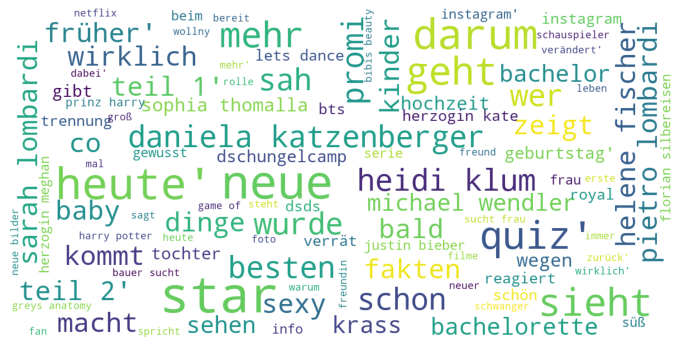
\includegraphics[width=10cm]{kapitel5/wo_click.png}
    \caption[Word Cloud Analyse für die Clickbaits Schlagzeilen]{Die Darstellung zeigt das Aufkommen der Häufigsten Wörter aus den Titeln der Clickbaits Nachrichten}
    \label{Kap5:clwc}
\end{figure}

\begin{figure}[H]
    \centering
    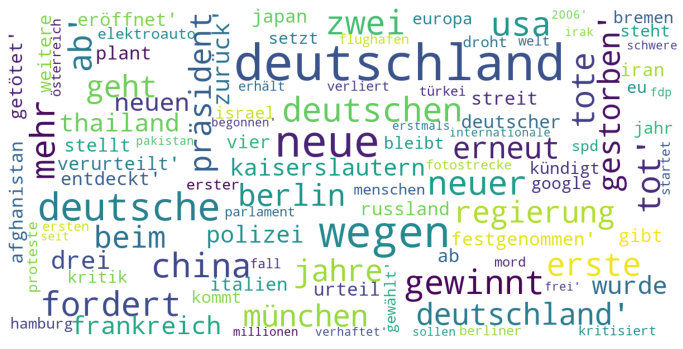
\includegraphics[width=10cm]{kapitel5/news.png}
    \caption[Word Cloud Analyse für die Wikinews Schlagzeilen]{Die Darstellung zeigt das Aufkommen der Häufigsten Wörter aus den Titeln der Wikinews Nachrichten}
    \label{Kap5:clwc}
\end{figure}
